\documentclass{article}
\usepackage[utf8]{inputenc}
\usepackage[spanish]{babel}
\usepackage{amsthm}
\usepackage{amssymb}
\usepackage{amsmath}
\usepackage{fancyhdr}
\usepackage{graphicx}
\usepackage[dvipsnames, table]{xcolor}
\usepackage[framemethod=tikz]{mdframed}
\usepackage{multicol}
\usepackage{tabularx}
\usepackage{pifont}
\setlength{\tabcolsep}{3pt}
\decimalpoint
\newcommand{\xmark}{\ding{55}}
\definecolor{mycolor}{rgb}{0.122, 0.435, 0.698}

\newmdenv[innerlinewidth=0.5pt, roundcorner=4pt,linecolor=mycolor,innerleftmargin=6pt,
innerrightmargin=6pt,innertopmargin=6pt,innerbottommargin=6pt]{mybox}


\setlength\parindent{0pt}

\newtheorem{definition}{Definición}
\newtheorem{proposition}{Proposición}

\renewcommand{\headrulewidth}{0.4pt}

\begin{document}
\date{13 - 20 marzo de 2020}
\title{ \textbf{Topología} \\
Semana 2: Conjuntos cerrados, puntos límite y espacios de Hausdorff}
%\author{Docente: Gabriel Chicas Reyes, MSc.\\ 
	%			Alumno: Kevin López Aquino }
\maketitle	

\begin{mybox}
\textbf{11. } Muestre que el producto de dos espacios de Hausdorff es Hausdorff. 	
\end{mybox}	
\begin{proof}
	Sean $X$ y $Y$ dos espacios de Hausdorff. Tomemos dos puntos $(x_{1}, y_{1}), (x_{2}, y_{2})$ distintos de $X \times Y$. Entonces, $x_{1} \neq x_{2}$ o $y_{1} \neq y_{2}$. Supongamos, sin pérdida de generalidad, que $x_{1} \neq x_{2}$. Puesto que $X$ es Hausdorff, podemos elegir entornos disjuntos $U_{1}, U_{2} \subseteq X$ de $x_{1}$ y $x_{2}$, respectivamente.  Entonces, $U_{1} \times Y$ y $(x_{2}, y_{2})$ son entornos de $(x_{1}, y_{1})$ y $U_{2} \times Y$, respectivamente, en la topología producto sobre $X \times Y$. Además, 
	$$ \left( U_{1} \times Y \right) \cap \left( U_{2} \times Y \right) =   \left( U_{1} \cap U_{2} \right) \times Y = \varnothing, $$
	con lo que queda demostrada la proposición. 
\end{proof}

\begin{mybox}
	\textbf{12. } Demuestre que un subespacio de Hausdorff es Hausdorff. 
\end{mybox}	
\begin{proof}
	Sea $X$ un espacio de Hausdorff y $Y$ un subespacio de este. Consideremos dos puntos distintos $x$ y $y$ en $Y$. Entonces, podemos encontrar abiertos $U, V$ de $X$ que contengan a $x$ y a $y$, respectivamente, y sean disjuntos. Se sigue que $Y \cap U$ y $Y \cap V$ son entornos de $x$ y de $y$, respectivamente, en el subespacio $Y$. Además, son entornos disjuntos: $(Y \cap U) \cap (Y \cap V) = Y \cap U \cap V = \varnothing.$
\end{proof}

\begin{mybox}
	\textbf{13. } Muestre que $X$ es Hausdorff si y solo si la \textbf{diagonal}
	$$ \Delta = \{ (x, x) \mid x \in X \} $$
	es cerrada en $ X \times X$.
\end{mybox}	
\begin{proof}
	$(\Leftarrow)$ Supongamos que $\Delta$ es cerrada en $X \times X$. Entonces, 
	$$ \left( X \times X \right)  \backslash \Delta = \{ (x, y) \in X \times X \mid x \neq y \}$$ 
es abierto en $X \times X$. Esto implica que para cualesquiera $x, y \in X$ tales que $x \neq y$, existen abiertos $U, V \subseteq X$ tales que
$$ (x, y) \in U \times V \subseteq  \left( X \times X \right)  \backslash \Delta. $$
De lo anterior se observa que no puede existir un elemento en $U \cap V$. Así, para $x$ y $y$ de $X$ distintos, hemos construido entornos disjuntos. Se sigue que $X$ es Hausdorff.\\
$(\Rightarrow)$ Ahora supongamos que $X$ es Hausdorff. Mostramos que $\left( X \times X \right)  \backslash \Delta$ es abierto. Si $(x, y) \in \left( X \times X \right)  \backslash \Delta$, deducimos que $x \neq y$ y que existen entornos disjuntos $U, V$ de $x$ y $y$, respectivamente. Notamos que $ (U \times V) \cap \Delta = \varnothing$, de forma que 
$$(x, y) \in U \times V \subseteq \left( X \times X \right)  \backslash \Delta.$$ 
Así, para cada punto en $\left( X \times X \right)  \backslash \Delta$ podemos encontrar un elemento básico dentro de este conjunto que lo contiene, de lo que se sique que $\left( X \times X \right)  \backslash \Delta$ es abierto. 
\end{proof}

\begin{mybox}
	\textbf{15. } Pruebe que el axioma $T_{1}$ es equivalente a la condición que para cada par de puntos distintos de $X$, cada uno posee un entorno que no contiene al otro. 
\end{mybox}	
\begin{proof}
	$(\Leftarrow)$ Supongamos que para par de puntos distintos de un espacio $X$, cada uno tiene un entorno que no contiene al otro. Demostraremos que todos los conjuntos unipuntuales son cerrados en $X$, de lo que se sigue que cualquier conjunto finito también será cerrado. \\
	Sea $x$ un punto de $X$. Mostramos que $\text{cl}\{x\} = \{x\}$. Consideremos un puntuo $y \neq x$. Por la hipótesis, podemos encontrar un entorno $V$ de $y$ tal que $x \notin V$; es decir, $V \cap \{x\} = \varnothing$. Así, hemos construido un entorno de $y$ que no interseca a $\{ x \}$, de lo que se sigue que $y \notin \text{cl}\{x\}$. Por tanto, $\text{cl}\{x\} = \{x\}$. \\
	$(\Rightarrow)$ Ahora supongamos que los subconjuntos finitos de $X$ son cerrados y tomemos dos puntos distintos $x$ y $y$ de $X$. Entonces, el conjunto $X \backslash \{y\}$ es un entorno de $x$ que no contiene a $y$. De manera similar, $X \backslash \{ x \}$ es un entorno de $y$ que no contiene a $x$.
\end{proof}
La parte $(\Leftarrow)$ sigue el mismo argumento de la demostración del \textbf{teorema 17.8} de \textbf{[1]}. Este hecho ilustra que no necesitamos algo tan fuerte como la propiedad de Hausdorff para que los conjuntos finitos sean cerrados: basta con una propiedad más débil como el axioma $T_{1}$. 
\newpage
\begin{figure}[h]
	\centering 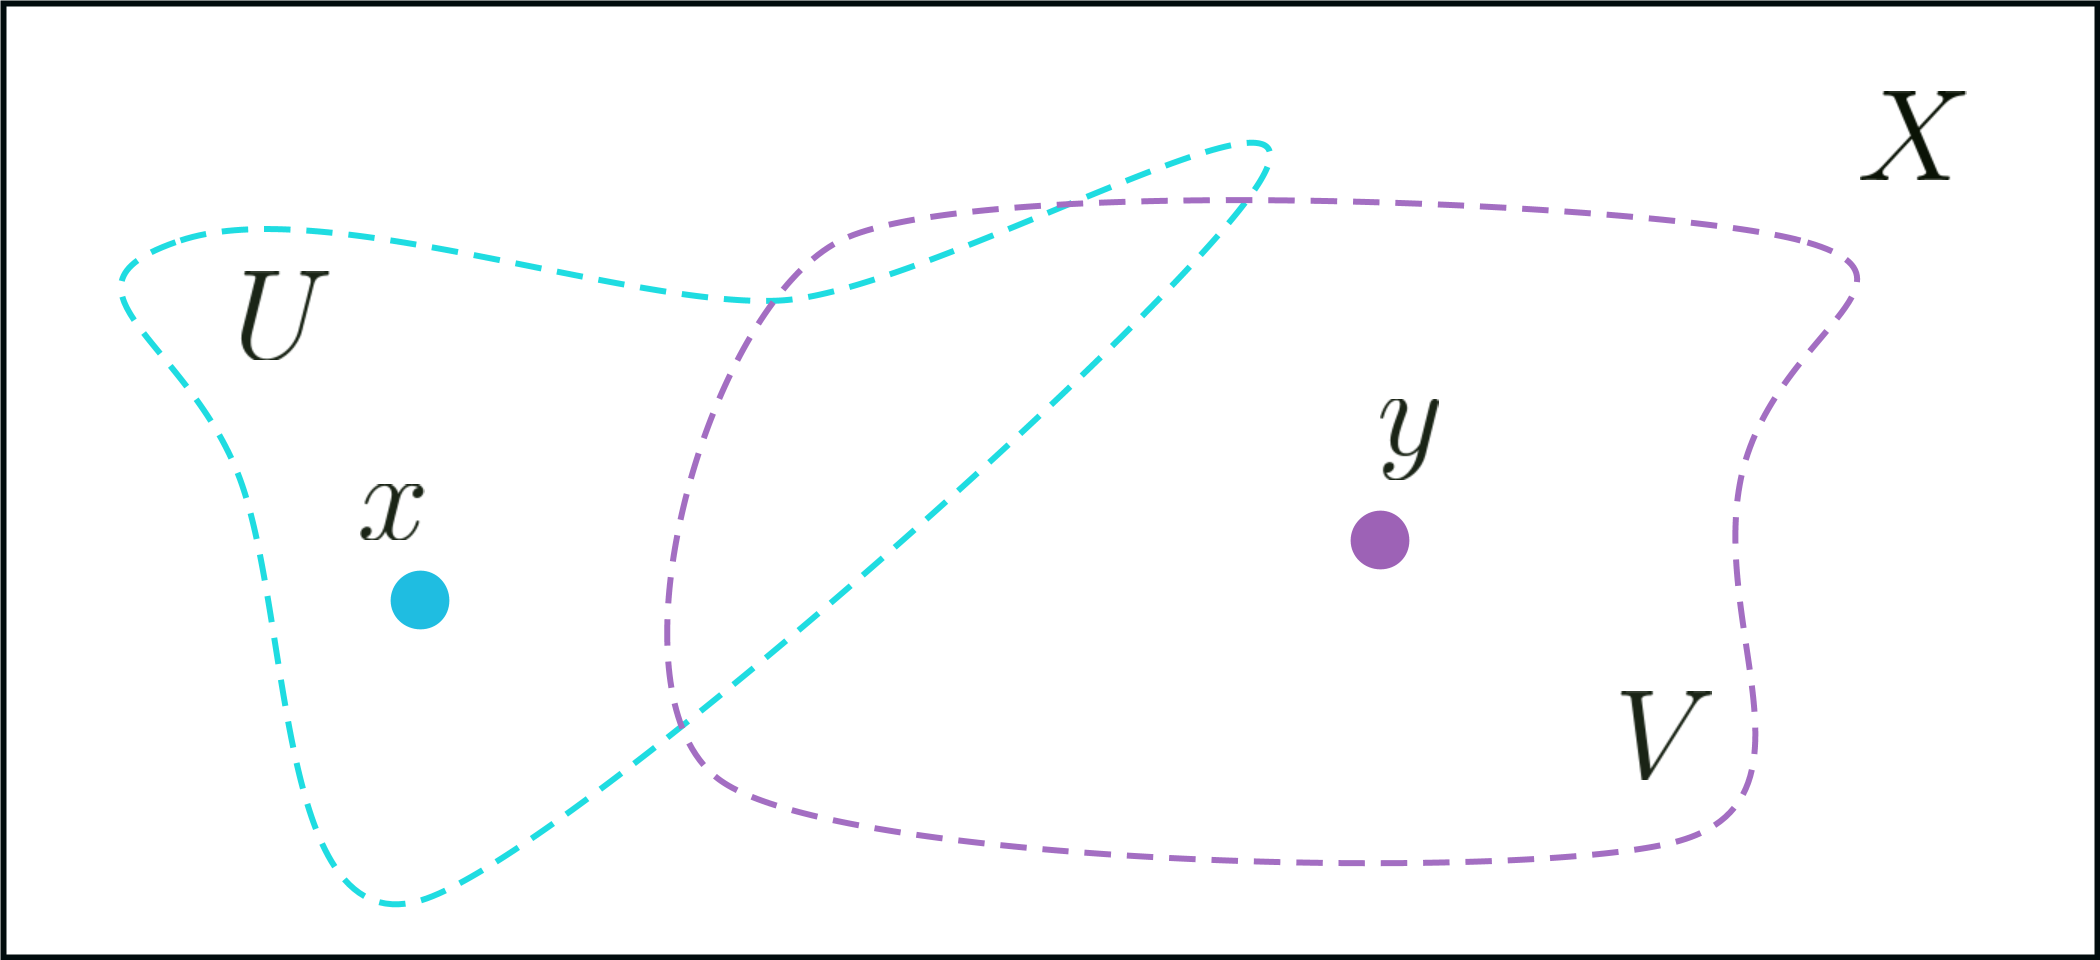
\includegraphics[scale=0.15]{e2fig.png}
	\caption{En un espacio $X$ que cumple el axioma $T_{1}$ siempre podemos hacer lo mostrado en la figura, pero no podemos garantizar que los entornos sean disjuntos, a diferencia de un espacio de Hausdorff. }
\end{figure}

\begin{mybox}
	\textbf{19. } Si $A \subseteq X$, definimos la \textbf{frontera} de $A$ mediante la ecuación
	$$ \partial A = \text{cl}(A) \cap \text{cl}(X \backslash A). $$
	\textbf{(a)} Pruebe que $\text{int}(A)$ y $\partial A$ son disjuntos y que $\text{cl}(A) = \text{int}(A) \cup \partial A$. \\
	
	\textbf{(b)} Muestre que $\partial A = \varnothing $ si y solo si $A$ es abierto y cerrado a la vez. 
\end{mybox}	
$\bullet$ Para ver que el interior de $A$ y su frontera son disjuntos, suponemos que existe un punto $x$ en ambos conjuntos. Al estar en el interior de $A$, se sigue que existe un $U$ entorno de $x$ contenido en $A$. Sin embargo, $x \in \text{cl}(X \backslash A)$, lo que implica que $U$ debe intersecar a $X \backslash A$. Teniendo en cuenta que $U \subseteq A$, esto resulta imposible. \\

Para demostrar que al unir el interior de un conjunto $A$ con su frontera obtenemos su clausura, primero notamos que la definición implica que $\partial A \subseteq \text{cl}(A)$. Además, sabemos que $\text{int}(A) \subseteq \text{cl}(A)$, de forma que $\text{int}(A) \cup \partial A \subseteq \text{cl}(A)$.\\
Para demostrar que $\text{cl}(A) \subseteq \text{int}(A) \cup \partial A$, supongamos que $x$ está en $\text{cl}(A)$ y no está en $\text{int}(A)$, con el fin de mostrar que $x \in \partial A$. Si tomamos un entorno arbitrario de $x$, notamos que no puede estar contenido en $A$, de forma que se debe intersecar con $X \backslash A$. Así, $x \in \text{cl}(X \backslash A)$, de lo que se sigue la conclusión. $\hspace*{\fill} \blacksquare$ \\

$\bullet \hspace{0.2cm} (\Leftarrow)$ Supongamos que $A$ es abierto y cerrado a la vez. Entonces, podemos decir lo mismo de $X \backslash A$. Usando el hecho que ambos conjuntos son cerrados, inferimos que 
$$ \text{cl}(X \backslash A) = X \backslash A \hspace{0.2cm} \text{y} \hspace{0.2cm} \text{cl}(A) = A.$$
Así, $ \partial A = A \cap (X \backslash A) = \varnothing.$   \\
$(\Rightarrow)$ Ahora supongamos que $\partial A = \varnothing.$ Por la parte $\textbf{(a)}$, se sigue que $\text{int} (A) = \text{cl}(A)$. En vista que $\text{int}(A) \subseteq A \subseteq \text{cl}(A)$, podemos deducir que $A = \text{int}(A) = \text{cl}(A)$, de forma que $A$ es abierto y cerrado. $\hspace*{\fill} \blacksquare$ \\

\begin{figure}[h]
	\centering 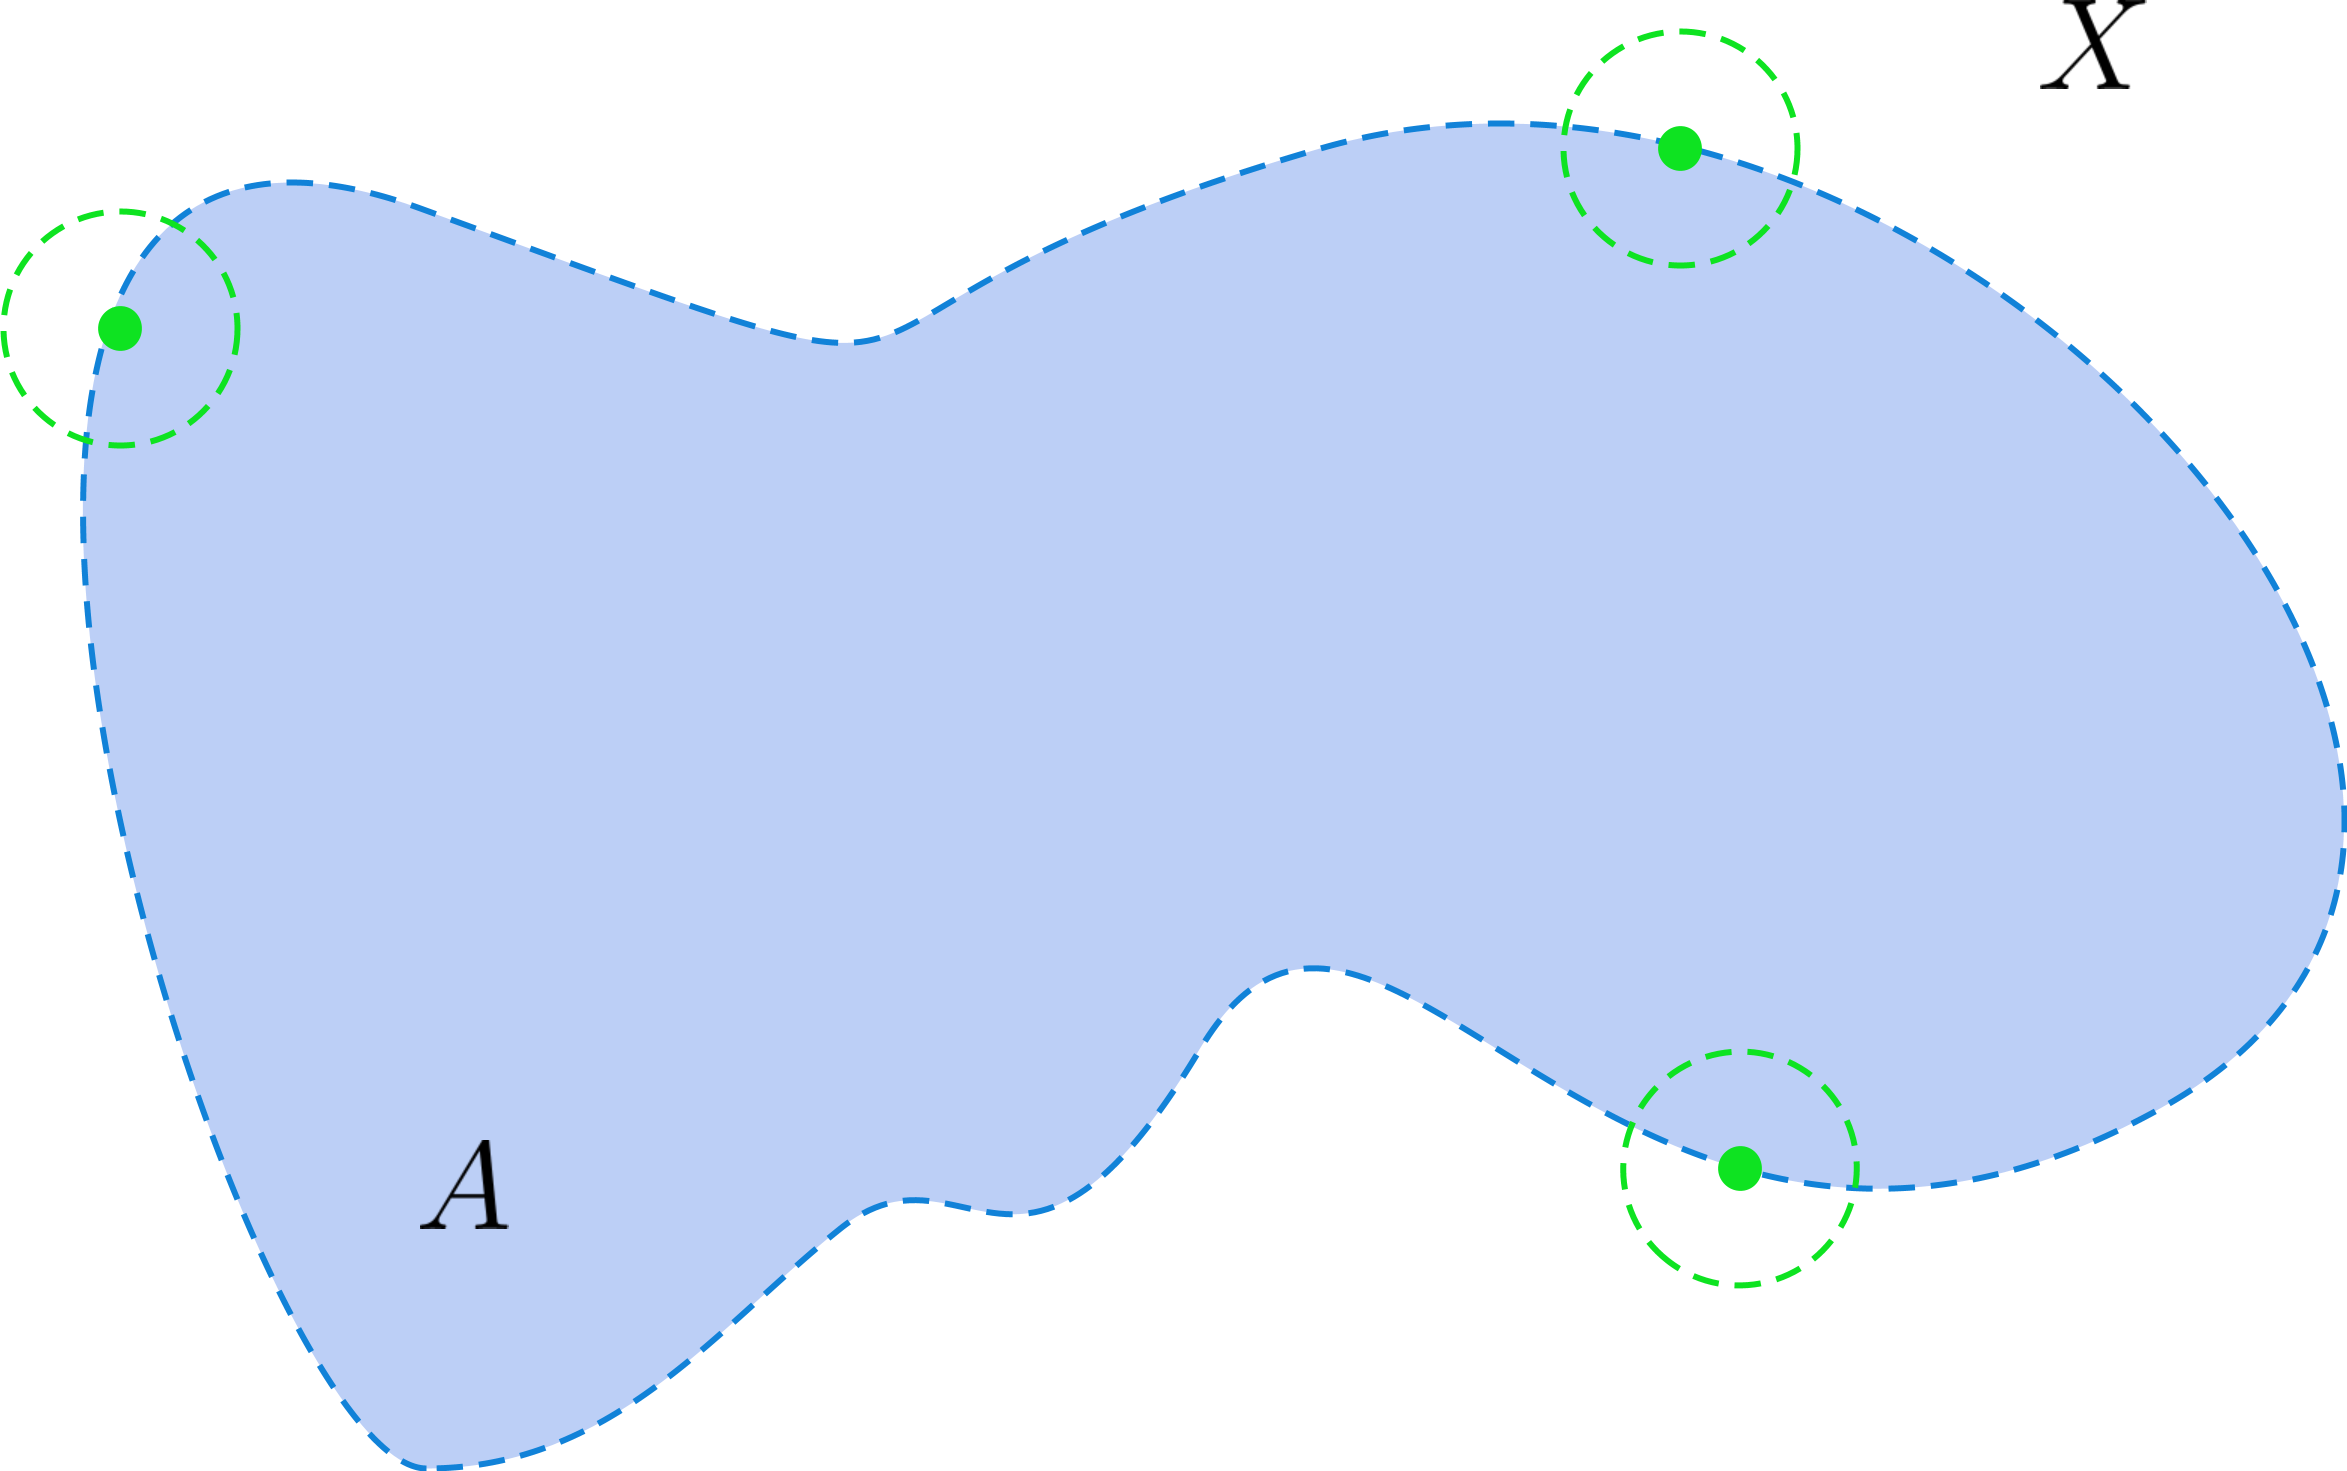
\includegraphics[scale=0.13]{e2fig2.png}
	\caption{Si un punto está en la frontera de $A$, cada entorno de ese punto contiene puntos dentro de $A$ y fuera de $A$. }
\end{figure}


\end{document}
